\newcommand\version{v1}
\problemname{Vänner}
$N$ vänner spelar ett spel. Spelet spelas på en rad med $L$ kvadrater, där kvadrat $i$ och $i+1$ är brevid varandra. Högst en vän står på varje kvadrat.
I varje drag i spelet hoppar en vän från sin kvadrat till en ny (tom) kvadrat.

Under varje tidpunkt i spelet är vännernas \emph{poäng} antalet vänner som har en vän antingen i rutan direkt till vänster eller rutan direkt till höger om vännen själv. Vid vissa tidpunkter kommer vännerna fråga vad deras nuvarande poäng är.

\section*{Exempel}
Antag att vi har $N = 3$ vänner som spelar på en av $L = 7$ kvadrater. Ursprungligen står dessa på platserna $1, 3, 4$. Poängen för denna position är $2$, eftersom vännerna på position $3$ och $4$ står brevid varandra.

Det första hoppet är från position $4$ till $2$, vilket ger oss positionerna $1, 2, 3$. I denna position har alla vänner någon brevid sig, så poängen är 3.

Det andra och sista hoppet är från $3$ till $0$, vilket resulterar i positionerna $0, 1, 2$. Alla vänner har fortfarande någon brevid sig, så poängen är fortfarande $3$.

\begin{figure}[h!]
  \centering
  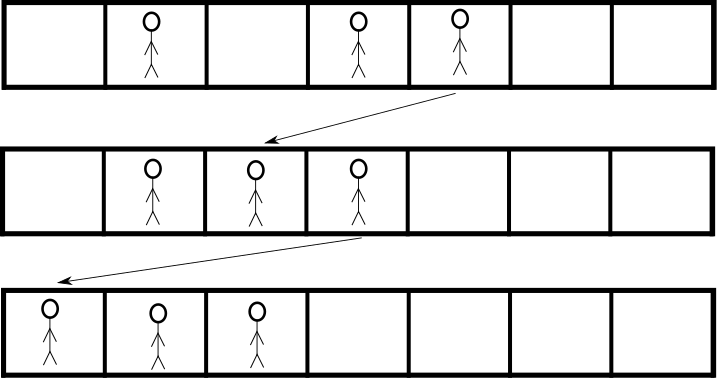
\includegraphics[width=0.8\textwidth]{sample.png}
  \caption{Illustration av exemplet}
\end{figure}

\section*{Uppgift}
Du kommer få samtliga hopp som görs i spelet, en efter en. Vid vissa tidpunkter kommer vännerna fråga vad deras nuvarande poäng är. Din uppgift är att implementera funktionerna 
\texttt{init(N, L, P)}, \texttt{jump(A, B)}, and \texttt{score()}:

\begin{itemize}
  \item \texttt{init(N, L, P)} - denna funktion anropas exakt en gång av domaren, i början av spelet.
  \begin{itemize}
    \item \texttt{N}: antalet vänner som spelar.
    \item \texttt{L}: antalet kvadrater i spelet.
    \item \texttt{P}: en vektor med $N$ element. \texttt{P[i]} ($0 \le i < N$) innehåller den ursprungliga
      positionen av den $i$:te vännen.
    \item Funktionen ska inte returnera något.
  \end{itemize}

  \item \texttt{jump(A, B)} - denna funktion anropas en gång för varje hopp, i den ordningen hoppen görs.
  \begin{itemize}
    \item \texttt{A}: positionen som vännen hoppar från 
      ($0 \le A < L$).
      Denna position innehåller alltid en vän när hoppet görs.
    \item \texttt{B}: positionen som vännen hoppar till
      ($0 \le B < L$).
      Denna position innehåller aldrig en vän när hoppet görs.
    \item Funktionen ska inte returnera något.
  \end{itemize}

  \item \texttt{score()} - denan funktion anropas när vännerna vill veta deras nuvarande poäng.
  \begin{itemize}
    \item Funktionen ska returnera den nuvarande poängen i spelet.
  \end{itemize}

\end{itemize}



\section*{Delpoäng}
Uppgiften består av ett antal grupper. Varje grupp ger ett visst antal poäng, och för att klara
gruppen måste du klara samtliga testfall i gruppen.

Låt $J$ vara antalet anrop till \texttt{jump} och $S$ antalet anrop till \texttt{score}.

\begin{tabular}{|l|l|l|}
  \hline
  \textbf{Grupp} & \textbf{Poäng} & \textbf{Gränser} \\ \hline
  1 & 9 & $1 \le N, L \le 1\,000$,  $S + J \le 2\,000$ \\ \hline
  2 & 17 & $1 \le N, L \le 100\,000$, $J = 0$, $S = 1$ \\ \hline
  3 & 14 & $1 \le N \le 100\,000$, $1 \le N \le 10^9$, $J = 0$, $S = 1$ \\ \hline
  4 & 38 & $1 \le N, L \le 100\,000$, $S + J \le 200\,000$ \\ \hline
  5 & 22 & $1 \le N \le 100\,000$, $1 \le N \le 10^9$, $S + J \le 200\,000$ \\ \hline
\end{tabular}

\section*{Indataformat}
Exempeldomaren läser indata i följande format:

\begin{itemize}
  \item rad 1: \texttt{N L Q}
  \item rad 2: \texttt{P[0] P[1] ... P[N - 1]}
  \item rad $3$ till $3 + Q - 1$: varje rad representerar antingen ett hopp eller en fråga om poängen.
    Om raden är \texttt{0 A B} ska ett hopp från $A$ till $B$ göras. Om raden är \texttt{1} frågar vännerna om poängen.
\end{itemize}

\section*{Utdataformat}
För varje fråga om poängen skriver exempeldomaren ut returvärdet av \texttt{score()}
